\chapter{Modulador 16-QAM}
\label{section:qam}


%aqui introduccion de qam y captura de los bloques



\section*{Mapeado 16-QAM}





%sacar los datos de la FIFO a 2MHz
%ráfagas de 200 datos

%En este ejemplo: (esto ya no, cambiar)
%Para la dimensión I, he asignado "000" a "-3", "001" a "-1", "010" a "1", y "011" a "3".
%Para la dimensión Q, he asignado "000" a "-3", "010" a "-1", "100" a "1", y "110" a "3".

La codificación Gray es una técnica específica que garantiza que solo un bit cambie entre dos valores consecutivos. Para modulación QAM, las tablas Q e I se ajustan para seguir la codificación Gray y minimizar la posibilidad de errores debido a cambios de múltiples bits en la transmisión.

\vspace{3mm}

    \begin{figure}[h]
    	\centering
    	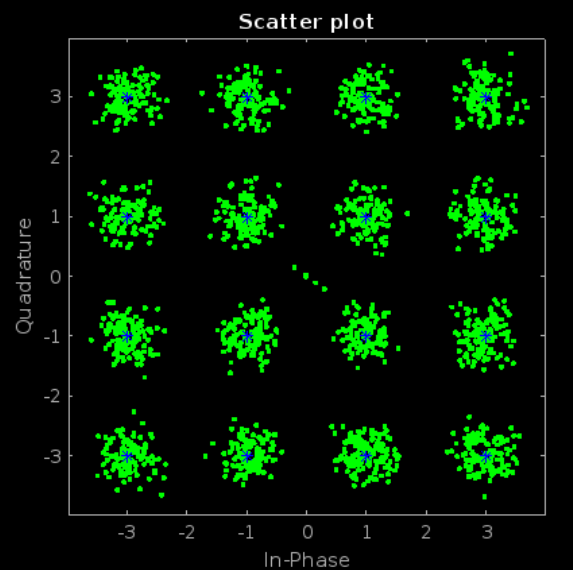
\includegraphics[width=0.5\textwidth]{img/matlab/qam.PNG}
    	\caption{}
    	\label{fig:qam}
    \end{figure}
    
\vspace{3mm}






\section*{Zero Padding}


\section*{Bloque de filtrado pulse shaping - RRC}



%193 coeficientes
%tenemos una ventana de 193 datos -> reg de desplazamiento (el actual+192 datos)
% y_filtro[t0] = sum193(y[ti]*coef[i])
%a la entrada hay valores enteros con signo(+1,-3,+3,-3)

%a=sfi(rrcfilter(1),16,16) %valor, nbits, nbits decimales)
%en este caso como los valores son de 0 con algo se ponen 16b decimales
%el error de precision es 2e-15/2 <- (1/2e-16)/2

%qr=sfi(rrcFilter',16)
%qr*2e17

%en freq response (en configuracion de vivado) coger gráfica
%config del filtro:
%se pone full precision 24, 3 bits signed

\vspace{3mm}

    \begin{figure}[h]
    	\centering
    	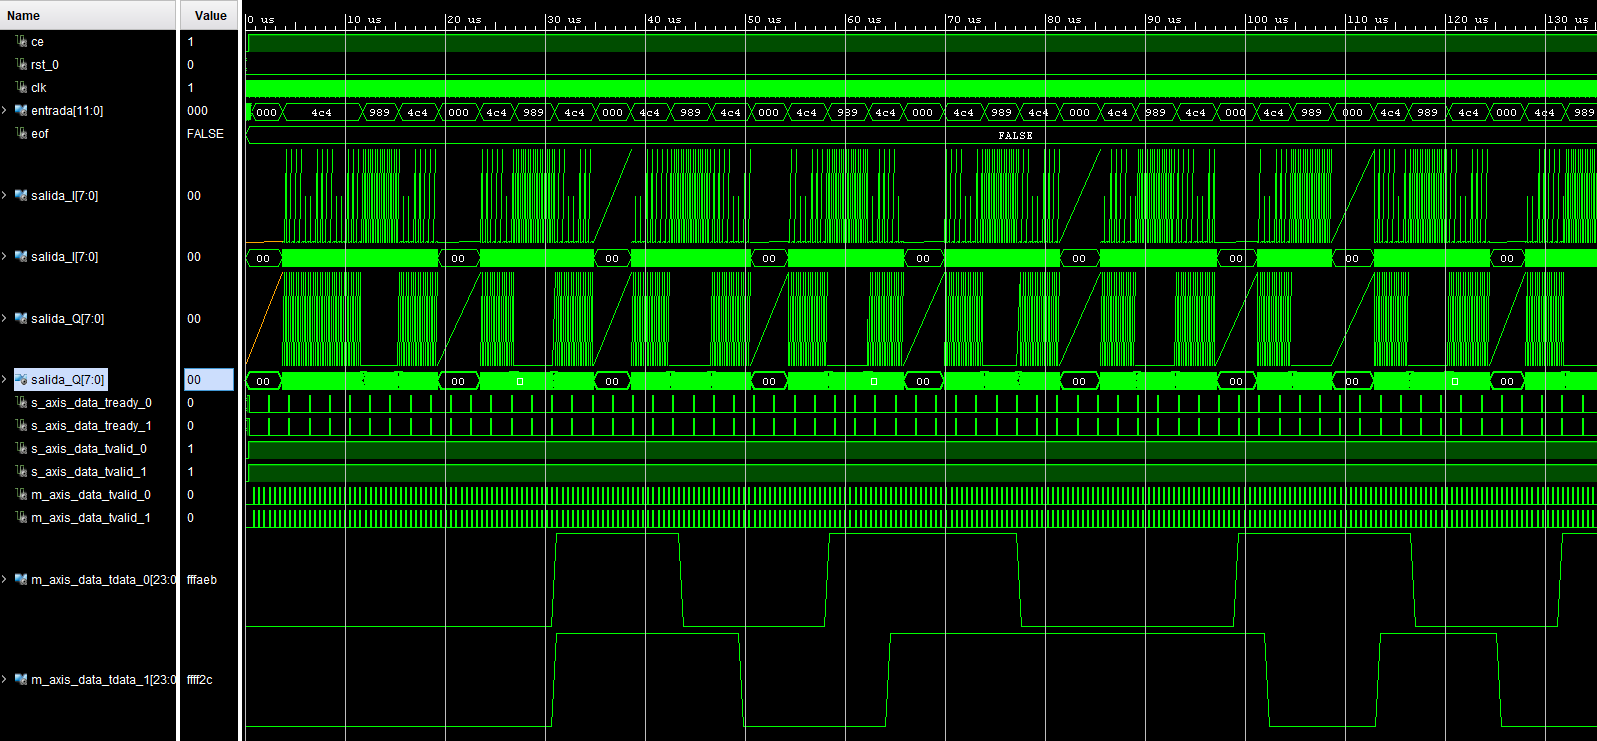
\includegraphics[width=1\textwidth]{img/matlab/rrc.PNG}
    	\caption{}
    	\label{fig:rrc}
    \end{figure}
    
\vspace{3mm}




\section*{Generación de las sinusoides coseno/-seno mediante bloque DDS a 576 MHz }